\documentclass[../../main]{subfiles}

\renewcommand\thesection{\arabic{section}}


\begin{document}

\section{Electronics Bay} \label{sec:}

\begin{figure}
    \centering
    \includegraphics [
        max width = \IGXMaxWidth,
        max height = \IGXMaxHeight,
        \IGXDefaultOptionalArgs,
    ] {tikzpics/endMiniProjectEMCU.pdf}
    \captionof{figure} {EMCU's electronics enclosure developed as part of Mini Project.}
    \label{fig:miniProjectEMCU}
\end{figure}

\alertCaution{
    Do not replicate the setup shown in Figure \ref{fig:miniProjectEMCU}. Most of
    the connections are made using fly wires from temporary, exposed insulated
    copper wires. While the maximum voltage in our case was only 12V, even this can
    cause damage or pose a safety risk if a short circuit occurs.
}

Figure \ref{fig:miniProjectEMCU} shows the electronics enclosure developed as part of Mini Project.
The first noticeable thing in figure \ref{fig:miniProjectEMCU} is the wires sticking out
everywhere. If you look closely, some of the connections are using insulated copper fly wires.
These wires can lose their insulation and can cause short circuits. Another thing is the connections
are soldered to each other in most areas. This makes debugging really tedious if something goes
south.

\begin{center}

    \begin{tabularx} {\textwidth} {
            >{\centering \arraybackslash}X
            >{\centering \arraybackslash}X
        }

        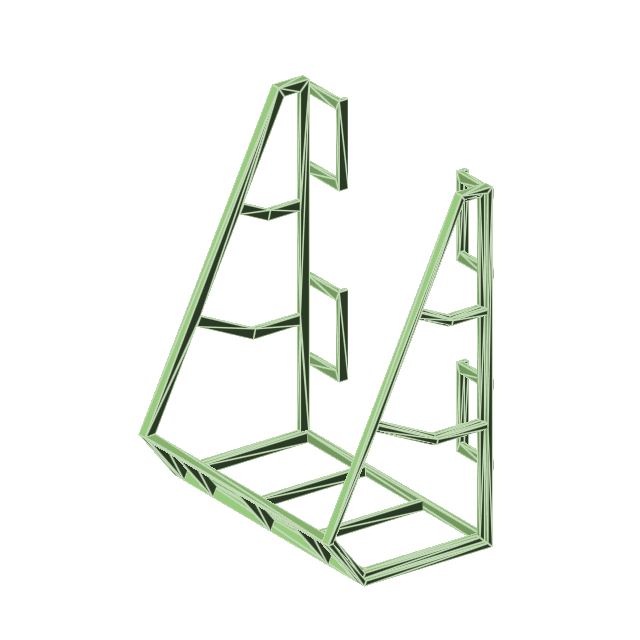
\includegraphics[
            height = 0.225\textheight,
        ] {../section_01/pics/elec_bay.png}

        &

        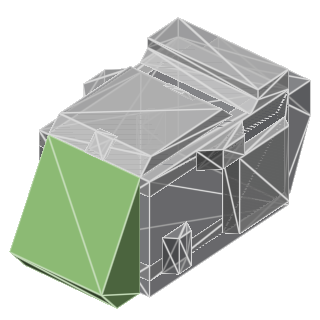
\includegraphics[
            height = 0.225\textheight,
        ] {pics/elec_bay_right.png}

        \\

    \end{tabularx}

    \captionof{figure}{Electronics bay structure CAD designs.}
    \label{fig:elecBayCAD}

\end{center}

Thus born the \emph{electronics bay}. Figure \ref{fig:elecBayCAD} shows the
structural design of the electronics bay. There won't be any fly wires in this
design, instead there will be a mother board and all the other board can be
connected to it using header pins. This helps to pull out each of the boards
for maintenance or debugging. Most of the electronic components, including the
power supply, will be housed in this bay, protecting them from water exposure
and temperature variations.

\end{document}
